% !TEX root = task-3-25-3.tex
% Editable task bank. Append new BankTask blocks at the end of the document.
\documentclass[12pt,a4paper]{article}
\usepackage{physics-textbook}
\usepackage{graphicx,needspace}
\usetikzlibrary{decorations.pathmorphing}
\newif\ifShowSolutions
\ifdefined\TutorEdition
  \ShowSolutionstrue
\else
  \ShowSolutionsfalse % Change to \ShowSolutionstrue to display solutions.
\fi
\newcounter{banktask}
\newsavebox{\BankTaskBox}
\newcommand{\BankTaskContent}[3]{%
  \noindent\textbf{\thebanktask.}\quad #2\par
  \ifShowSolutions
    \Needspace{50mm}% Keep the solution heading with its opening text or diagram.
    #3\par
    \ifdefined\TutorEdition
      \ifcsname TutorSource#1\endcsname
        \nopagebreak\smallskip{\small\csname TutorSource#1\endcsname\par}%
      \fi
    \fi
  \fi
}
\newcommand{\BankTask}[3]{%
  \refstepcounter{banktask}\par\medskip
  \sbox{\BankTaskBox}{\begin{minipage}{\linewidth}%
    \BankTaskContent{#1}{#2}{#3}\end{minipage}}%
  \ifdim\dimexpr\ht\BankTaskBox+\dp\BankTaskBox\relax>\dimexpr\textheight-20mm\relax
    \Needspace{35mm}\BankTaskContent{#1}{#2}{#3}%
  \else
    \Needspace{\dimexpr\ht\BankTaskBox+\dp\BankTaskBox\relax}%
    \noindent\usebox{\BankTaskBox}\par
  \fi
  \medskip
}
\begin{document}
\BookSubsection{3.25.3}{Трансформатор}


% Source 2928: https://phys-ege.sdamgia.ru/problem?id=2928
\BankTask{2928}{
На рисунке приведена электрическая цепь, состоящая из гальванического элемента, реостата, трансформатора, амперметра и вольтметра.
\begin{center}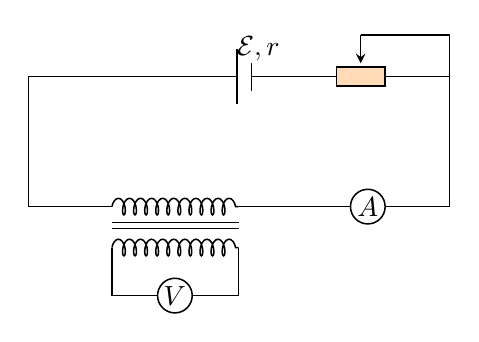
\begin{tikzpicture}[>=stealth,line width=.55pt]\draw(0,0)--(0,1.65)--(2.65,1.65) (2.83,1.65)--(5.35,1.65)--(5.35,0)--(2.67,0) (1.06,0)--(0,0);\draw(2.65,1.3)--(2.65,2) (2.83,1.47)--(2.83,1.83);\node[above]at(2.92,1.72){$\mathcal E,r$};\draw[->](4.22,2.18)--(4.22,1.82);\draw(4.22,2.18)--(5.35,2.18)--(5.35,1.65);\draw[decorate,decoration={coil,aspect=.45,amplitude=3pt,segment length=4pt}](1.06,0)--(2.67,0);\draw(1.06,-.2)--(2.67,-.2) (1.06,-.28)--(2.67,-.28);\draw[decorate,decoration={coil,aspect=.45,amplitude=3pt,segment length=4pt}](1.06,-.52)--(2.67,-.52);\draw(1.06,-.52)--(1.06,-1.13)--(2.67,-1.13)--(2.67,-.52);\draw[fill=orange!28](3.9099999999999997,1.5299999999999998)rectangle(4.529999999999999,1.77);\node[above]at(4.22,1.77){$$};\draw[fill=white](4.31,0)circle(.22)node{$A$};\draw[fill=white](1.86,-1.13)circle(.22)node{$V$};\end{tikzpicture}\end{center}
В начальный момент времени ползунок реостата установлен посередине и неподвижен. Опираясь на законы электродинамики, объясните, как будут изменяться показания приборов в процессе перемещения ползунка реостата вправо. ЭДС самоиндукции пренебречь по сравнению с $\mathcal E.$
}{
\smallskip\noindent\textbf{Решение}\par
$1$.  Во время перемещения движка реостата показания амперметра будут плавно уменьшаться, а вольтметр будет регистрировать напряжение на концах вторичной обмотки. Примечание: для полного ответа не требуется объяснения показаний приборов в крайнем правом положении. (Когда движок придет в крайнее правое положение и движение его прекратится, амперметр будет показывать постоянную силу тока в цепи, а напряжение, измеряемое вольтметром, окажется равным нулю.)
$2$.  При перемещении ползунка вправо сопротивление цепи увеличивается, а сила тока уменьшается в соответствии с законом Ома для полной цепи: $I= \frac{\mathcal E}{R + r} ,$ где R  — сопротивление внешней цепи.
Изменение тока, текущего по первичной обмотке трансформатора, вызывает изменение индукции магнитного поля, создаваемого этой обмоткой. Это приводит к изменению магнитного потока через вторичную обмотку трансформатора. В соответствии с законом индукции Фарадея возникает ЭДС индукции $\mathcal E = - \frac{\Delta \Phi}{\Delta t}$ во вторичной обмотке, а следовательно, напряжение U  на ее концах, регистрируемое вольтметром.
}

\end{document}
